\documentclass[authoryear,11pt]{elsarticle}

%This eliminates the `Preprint submitted to...' footer on the first page
\makeatletter
\def\ps@pprintTitle{%
 \let\@oddhead\@empty
 \let\@evenhead\@empty
 \def\@oddfoot{}%
 \let\@evenfoot\@oddfoot}
\makeatother

\usepackage{amssymb}
\usepackage{amsthm}
\usepackage{caption}
\usepackage{amsmath}
\usepackage{morefloats}
\usepackage{bbm}        %To allow \mathbb{1}

\usepackage{rotating}   %To turn tables sidewaystable
\usepackage{graphicx}
\usepackage{setspace}
\usepackage{hyperref}

%\onehalfspacing

\setlength{\parindent}{0pt}

\usepackage[top=3.5cm,bottom=3.75cm,left=2.45cm,right=2.45cm]{geometry}% by courtesy of Mico

\begin{document}
\begin{frontmatter}
\title{MFE Economics\\Problem set 2}
\end{frontmatter}

%%%%%%%%%%%%%%%%%%%%%%%%%%%%%%%%%%%%%%%%%%%%%%%%%%%%%%%%%%%%%%%%%%%%%%%%%%%%%%%%%%%%%%%%%%%%%%%%%%%%%%%%%%%%%%%%%%%%%%%%%%%%%%%%%%%%%%%%%%%%%%%%%%%%%%%%
%%%%%%%%%%%%%%%%%%%%%%%%%%%%%%%%%%%%%%%%%%%%%%%%%%%%%%%%%%%%%%%%%%%%%%%%%%%%%%%%%%%%%%%%%%%%%%%%%%%%%%%%%%%%%%%%%%%%%%%%%%%%%%%%%%%%%%%%%%%%%%%%%%%%%%%%

\section{Deriving the PV budget constraint}
In class we had the flow budget constraint of the form below\footnote{As someone pointed out in the lecture, it's sort of overcomplicating things by carrying around $t$ to mean a generic period - why not simply assume $t=0$ and get on with it. It's basically because we want to emphasize that these flow budget constraints do apply generically, in all periods.}
\begin{equation}
a_{t+s+1} = R_{t+s} a_{t+s} + y^{i}_{t+s} - c^{i}_{t+s} \; \forall s \geq 0 \label{eqn:flow}
\end{equation}
\begin{enumerate}
\item	In period $t+s-1$ you previously decided what your wealth, $a_{t+s}$, should be in your `bank account' at the end of that period.
\item	On entering period $t+s$ your wealth from the previous period earns the gross interest rate, $R_{t+s}$, meaning you have $R_{t+s} a_{t+s}$ before you receive your endowment $y_{t+s}$ and purchase consumption, $c_{t+s}$ in period $t+s$.
\item	Your savings in period $t+s$ (or if negative, dissavings) are $y_{t+s} - c_{t+s}$ which, combined with the wealth $R_{t+s} a_{t+s}$ will determine the wealth at the end of $t+s$, $a_{t+s+1}$, which you carry forward into $t+s+1$.
\item	Go to the next period and we're back to the start of the loop, but one period in the future.
\end{enumerate}

\begin{itemize}
\item	Rearrange equation \ref{eqn:flow} to have $a_{t+s}$ on the LHS and everything else on the right
\item	Assume that we start in $t=0$ (let's just get rid of $t$ for now by assuming it's period `0')
\item	By repeatedly substituting for future values of $a$ (keep using the next period version of the equation you just derived, to eliminate  wealth from the RHS) show that\footnote{Hint: Do it for the first few periods, rearrange terms/tidy up and you'll see the pattern emerging\ldots Also, note that the $\tilde{R}$ thing is just a multi-period PV discount allowing for possibly varying $R_{s}$.}
\begin{eqnarray}
a_{0} + \sum\limits_{s=0}^{T-1} \frac{y_{s}}{\tilde{R}_{s}} &=& \frac{1}{\tilde{R}}a_{T} + \sum\limits_{s=0}^{T-1} \frac{c_{s}}{\tilde{R}_{s}} \label{eqn:pv_bc_T} \\
\tilde{R}_{K} &\equiv& \prod\limits_{s=0}^{K} R_{s} \label{eqn:pv_bc_T}
\end{eqnarray}
\item	In class, we discussed a TVC that means that, as $T\rightarrow\infty$, the $\frac{1}{\tilde{R}}a_{T}$ terms is taken to be zero and we obtain the infinite horizon \textit{present value budget constraint}, below:
\begin{equation}
a_{0} + \sum\limits_{s=0}^{\infty} \frac{y_{s}}{\tilde{R}_{s}} = \sum\limits_{s=0}^{\infty} \frac{c_{s}}{\tilde{R}_{s}} \label{eqn:pv_bc_infty}
\end{equation}
\item	For finite $T$ and assuming $a_{0}$ was positive, what does a negative $a_{T}$ imply about the general relationship between $y$ and $c$ in the intervening periods? What does it imply about the relationship in any single period (assuming $T>1$)?
\item	If $$a_{0} + \sum\limits_{s=0}^{T} \frac{y_{s}}{\tilde{R}_{s}} < \sum\limits_{s=0}^{T} \frac{c_{s}}{\tilde{R}_{s}}$$ then, using equation (\ref{eqn:pv_bc_infty}), show that implies equation (\ref{eqn:pay_piper}) below. Interpret what that means for the general relationship between the PV of $y$ and $c$ from $T+1$ onwards? Relate it to the phrase `pay the piper'.
\begin{equation}
\sum\limits_{s=T+1}^{\infty} \frac{y_{s}}{\tilde{R}_{s}} > \sum\limits_{s=T+1}^{\infty} \frac{c_{s}}{\tilde{R}_{s}} \label{eqn:pay_piper}
\end{equation}
\end{itemize}

\subsection*{Answers}
Suppressing $i$,
\begin{equation*}
a_{t+s+1} = R_{t+s} a_{t+s} + y_{t+s} - c_{t+s}
\end{equation*}
implies
\begin{eqnarray*}
a_{t+s} &=& R^{-1}_{t+s} a_{t+s+1} - R^{-1}_{t+s} X_{t+s} \\
X &\equiv& y_{t+s} - c_{t+s}
\end{eqnarray*}
Taking $t=0$ we have
\begin{equation}
a_{s} = R^{-1}_{t+s} a_{t+s+1} - R^{-1}_{t+s} X_{t+s} \label{eqn:flow_s}
\end{equation}
Then, considering the $s=0$ case
\begin{equation}
a_{0} = R^{-1}_{0} a_{1} - R^{-1}_{0} X_{0} \label{eqn:flow_s_0}
\end{equation}
But since equation(\ref{eqn:flow_s}) holds for $s=1$ too, we have
\begin{equation*}
a_{1} = R^{-1}_{1} a_{2} - R^{-1}_{1} X_{1} \label{eqn:flow_s_1}
\end{equation*}
which can be substituted into equation (\ref{eqn:flow_s_0}) yielding
\begin{eqnarray*}
a_{0} 	&=& R^{-1}_{0} (R^{-1}_{1} a_{2} - R^{-1}_{1} X_{1}) - R^{-1}_{0} X_{0} \\
		&=& \frac{1}{R_{0}R_{1}} a_{2} - \frac{1}{R_{0}} X_{0} - \frac{1}{R_{0}R_{1}} X_{1}
\end{eqnarray*}
Repeat the process of substituting for assets on the right hand side and you obtain
\begin{eqnarray*}
a_{0} 	&=& \frac{1}{\tilde{R}_{s}}a_{T+1} - \sum\limits_{s=0}^{T} \frac{1}{\tilde{R}_{s}} X_{s} \\
\tilde{R}_{t}	&\equiv& \prod\limits_{s=0}^{t} R_{s}
\end{eqnarray*}
or, recalling the definition of $X_{t}$
\begin{equation*}
a_{0} + \sum\limits_{s=0}^{T} \frac{y_{s}}{\tilde{R}_{s}}	 = \frac{a_{T+1}}{\tilde{R}_{s}} + \sum\limits_{s=0}^{T} \frac{c_{s}}{\tilde{R}_{s}}
\end{equation*}

If you started with positive $a_{0}$ and $a_{T}<0$ then it means that you've run down your wealth from a positive to a negative net worth position. This implies that the value of your expenditures has exceeded that of your income, when discounted back to time $0$ dollars. Basically, you've been borrowing so much that you've become a net debtor. That doesn't necessarily mean that in every period your expenditure has exceeded income, just that typically it has done.

Subtract the equation from the PV budget constraint. This cancels out $a_{0}$ and all the discounted income and expenditure terms from $T$ and earlier, leaving the `tail' from $t=T+1$ to $\infty$ (the infinite future). The first inequality then immediately implies the second. If you've been spending beyond your means over the first $T$ periods, you're going to have to spend within your means (i.e. start saving) in the remaining periods on `average' (though not necessarily in every period). You've enjoyed the piper's music at the party but eventually you've got to pay him/her. This stems from our assumption that the PC budget constraint must be satisfied.



\section{Optional question: CRRA utility}
The Arrow-Pratt measure of absolute risk aversion for an agent with preferences representable using a suitably differentiable felicity function, $u(\cdot)$ pre is given by
\[
A(c) = - \frac{u''(c)}{u'(c)}
\]
where $u'(\cdot)$ indicates the first derivative of $u$ and $u''(\cdot)$, the second.

The Arrow-Pratt measure of relative risk aversion for such an agent is given by
\[
R(c) = c \times A(c)
\]

Calculate these two measures of risk aversion for an agent with felicity function
\[
u(c) = \frac{c^{1-\sigma} - 1}{1-\sigma}
\]
This function is typically used whenever one discusses relative risk aversion and it is referred to as a `constant relative risk aversion' (CRRA) preference specification. Why does it have this name?

Also, calculate relative risk aversion for an agent with a similar felicity function
\[
u(c) = \frac{c^{1-\sigma}}{1-\sigma}
\]
Compare to your previous answer and comment (very) briefly.

\subsection*{Answers}
\begin{eqnarray*}
u'(c) &=& c^{-\sigma} \\
u''(c) &=& -\sigma c^{-\sigma - 1}
\end{eqnarray*}

We have that $R(c) = \sigma$ and $A(c)=\frac{\sigma}{c}$ in both cases since $u(c)$ differs by a shift of $-\frac{1}{1-\sigma}$, which does not change any of the derivatives involved.

\section{Optional question (for revision/background): CRRA and Log Utility}
L'Hopital's rule states (roughly) that, if\ldots
\begin{itemize}
\item	$\lim_{x \to c} f(x) = \lim_{x \to c} g(x)=0$
\item	$g'(x)\neq0$
\item	$\lim_{x \to c} \frac{f'(x)}{g'(x)}$ exists
\end{itemize}
then
\[
\lim_{x \to c} \frac{f(x)}{g(x)} = \lim_{x \to c} \frac{f'(x)}{g'(x)}
\]

Frequently, you will find papers that say something like, we consider an agent with CRRA preferences $u(c) = \frac{c^{1-\sigma} - 1}{1-\sigma}$ for $\sigma>1$ and $u(c) = \log{(c)}$ for the case of $\sigma=1$. It is not immediately obvious (to most people) why this should make sense as $\sigma$ does not seem to appear in any meaningful way. The reason is that $\log{(c)}$ is the limit of $\frac{c^{1-\sigma} - 1}{1-\sigma}$ as $\sigma \rightarrow 1$. Use L'Hopital's rule to show this.\footnote{Hint: rewrite $C_{t}$ as $e^{\log{(C_{t})}}$ in the CRRA utility function.} Referring to the previous question, why, therefore do we tend to have the $-1$ in the definition of the CRRA felicity function, despite your answer to the final bit of that question?

\subsection*{Answers}
Think of the utility function as being a function of $\sigma$ (for any given $C$). In fact, think of it being a ratio of functions, $f$ and $g$ where
\begin{eqnarray*}
f(\sigma) \equiv C^{1-\sigma} - 1 \\
g(\sigma) \equiv 1 - \sigma
\end{eqnarray*}

We see that both $f(\sigma)$ and $g(\sigma)$ go to zero as $\sigma \to 1$. Furthermore, $g'(\sigma)=-1$ which is non-zero for all values of $\sigma$. Thus, two of the three conditions for use of L'Hopital's rule hold here. Now consider the ratio of derivatives, $f'(\sigma)/g'(\sigma)$. Before we do this, it is useful to re-express $f$ as follows
\[
f(\sigma) = C^{1-\sigma} - 1 \equiv e^{(1-\sigma)\log{(C)}}-1
\]
Thus the derivative of $f$ with respect to $\sigma$ is (remember the notes on how to differentiate exponentials) as follows\footnote{The relevant rule here is \[\frac{d}{dx}e^{f(x)} = f'(x)e^{f(x)}\]}
\[
f'(\sigma) = -\log{(C)} e^{(1-\sigma)\log{(C)}}
\]
Consequently, we have the ratio of derivatives
\[
\frac{f'(\sigma)}{g'(\sigma)} = \log{(C)} e^{(1-\sigma)\log{(C)}}
\]
The limit of this ratio as $\sigma \to 1$ exists and is equal to $\log{(C)}$ (since $e^{0}=1$) but by L'Hopital this means that the limit of our utility function is, in fact, a log utility function. Note that the $-1$ in the previous question means that the function values align in the limit (regardless of the marginal utilities aligning).


\section{GE model with CRRA felicity}
Review the arguments in the second lecture showing that the market interest rate in the GE model with heterogenous endowments (possibly different ${y_{t}^{i}}_{i=1:N}$ for different people $i$) is equal to the market interest rate in a GE model with a representative agent who receives an endowment process equal to $y_{t}=\sum\limits_{i=1}^{N}y_{t}^{i}$. The general equilibrium result in class (the endowment economy case) assumed that felicity was logarithmic in consumption. Will the market rate of interest be the same in GE models with and without heterogeneity if the felicity function is of the CRRA form $u(c_{t}^{i})=\frac{(c_{t}^{i}-1)^{1-\sigma }}{1-\sigma }$?

\subsection*{Answers}
The maximisation problem of agent $i$ is
\[
\max_{\{c_{t+s}^{i},a_{t+s+1}^{i} \}} \sum\limits_{s=0}^{\infty} \beta^{s} \frac{(c_{t+s}^{i}-1)}{1-\sigma}
\]
subject to a TVC and flow budget constraints discussed in class. The FOC (first order condition) with respect to assets is
\[
(c_{t}^{i})^{-\sigma} = \beta R_{t+1} (c_{t+1}^{i})^{-\sigma}
\]
which implies
\[
c_{t}^{i} = (\beta R_{t+1})^{-\frac{1}{\sigma}}c_{t+1}^{i}
\]
Aggregating (summing) across individuals we obtain
\[
\sum\limits_{i}c_{t}^{i} = (\beta R_{t+1})^{-\frac{1}{\sigma}}\sum\limits_{i}c_{t+1}^{i}
\]
and market clearing requires
\[
\sum\limits_{i}c_{t}^{i} = \sum\limits_{i}y_{t}^{i} \equiv y_{t}
\]
where $y_{t}$ is aggregate output.\footnote{You could also imagine a representative (maybe this is a more natural interpretation) agent consuming the `average' endowment ,rather than the whole aggregate endowment, in which case think of $y_{t}$ as $n \bar{y}_{t}$ where $\bar{y}_{t}$ is the average of the $y_{t}^{i}$. All the $n$'s will drop out in the following expressions though. When you're working with a representative agent, almost by definition, aggregate and average are bound together.}

Combining these relations, as in class, we obtain the same conditions that would emerge from an economy with a representative household but who obtains the aggregate/average endowment from the multiple agent economy.



\section{Optional question (for revision): Elasticities}
As a quick refresher, if we have a function $f(x)$ then its \href{https://en.wikipedia.org/wiki/Elasticity_of_a_function}{\textbf{elasticity}} with respect to $x$ is defined as
\[
 \frac{x}{f(x)} \frac{df(x)}{dx}
\]
which gives the percentage change in $f$ for a percentage change in $x$ (for small changes). In fact, one can alternatively calculate it as
\[
\frac{d \log{(f(x))}}{d \log{(x)} }
\]

Now, consider the production function of firm $i$
\[
Y_{i,t} = A_{t} N_{i,t}^{1-\alpha}
\]
What is the elasticity of output with respect to labor?

\subsection*{Answers}
We have that
\[
\frac{dY_{i,t}}{dN_{i,t}} = (1-\alpha)A_{t}N_{i,t}^{-\alpha}
\]
so that
\begin{eqnarray*}
\frac{N_{i,t}}{Y_{i,t}}\frac{dY_{i,t}}{dN_{i,t}} &=& (1-\alpha)A_{t}N_{i,t}^{-\alpha} \frac{N_{i,t}}{Y_{i,t}} \\
&=& (1-\alpha)A_{t}N_{i,t}^{1-\alpha} \frac{1}{A_{t} N_{i,t}^{1-\alpha}} \\
&=& 1-\alpha
\end{eqnarray*}

Alternatively, we could have used the derivation involving log versions (lower case) of the variables
\[
\frac{d}{dn_{i,t}} \log{(y_{i,t})} = \frac{d}{dn_{i,t}} (a_{t} + (1-\alpha)n_{i,t}) = 1-\alpha
\]

\section{CRRA and Elasticity of Intertemporal Substitution}
Using the Euler equation from a CRRA agent
\[
1 = \beta R \left( \frac{c_{t+1}}{c_{t}} \right)^{-\sigma}
\]
Show that the elasticity of $G_{c,t+1} \equiv \frac{c_{t+1}}{c_{t}}$ with respect to $R$ is $\frac{1}{\sigma}$. Note that we are in a riskless case here (hence the absence of an expectation operator in the Euler equation). Comment on the appearance and interpretation of $\sigma$ in the elasticity, given the absence of risk in this case.

\subsection*{Answers}
Rearrange to obtain
\[
c_{t}^{-\sigma} = \beta R c_{t+1}^{-\sigma}
\]
and then
\[
c_{t} = (\beta R)^{-\frac{1}{\sigma}} c_{t+1}
\]
or
\[
G_{c,t+1} = \beta^{\frac{1}{\sigma}} R^{\frac{1}{\sigma}}
\]
Take logs of each side and ignore the constant
\[
\log{(G_{c,t+1})} = const + \frac{1}{\sigma} \log{(R)}
\]
We see that although $\sigma$ was shown (see earlier questions) to be the CRRA, it does double duty in determining the EIS. Thus we have the (undesirable) property that an agent's attitudes to two different phenomena (smoothing consumption across stochastic contingencies vs. smoothing consumption across time) are bound together. This property is relaxed under Epstain-Zin preferences, for those of you who are interested.

\section{Pricing with market power}
\textbf{[RB: This question is to give you a head start on some NK stuff in a non-NK setting]}

In the NK model we are about to cover in class, we assume that firms exist in a situation of `monopolistic competition'. Without delving into the details of monopolistic competition (see various lecture notes available all over the web) what is important for our purposes is that the firms have some pricing power - they can vary their price marginally and thereby induce marginal changes in demand for their good. People sometimes refer to this as `facing a downward sloping demand curve'.\footnote{This is in contrast to the perfect competition case where firms take prices as given and if their price - somehow - ever deviated from that price, they would lose all demand or absorb the whole market, neither of which is sustainable in an equilibrium. Thus they effectively face a `horizontal' demand curve at whatever the competitive market price is.} If the firm wants to sell more, it must cut its price and if it wants to sell less, it must raise its price. Ultimately, then, their profit maximizing decision about the scale of operation (and implicitly employment etc.) comes down to choosing a price. They are price setters, not price takers.

In monopolistic competition, people normally have in mind a situation in which each monopolist produces a particular good that is somewhat differentiated but also somehow similar to goods produced by the other monopolists. The fact that the goods are different but somewhat substitutable means that raising the price may drive people towards the other goods. For example, a firm may have a monopoly in producing soft drink `x' but if they raise the price, that partly leads people to substitute towards soft drink `y' (a similar, if differentiated, good).\footnote{An important element of `competition' comes from firms entering or exiting the industry until expected profits from entry are zero - but we ignore this industrial organization stuff\ldots}

In the NK model, you will see that the particular structure of household preferences where the consumer gets utility from a bundle of different consumption goods gives rise to a degree of substitutability across goods, which is reflected in the demand curve for each of the different goods. These curves show that demand is decreasing in the goods' relative price where the steepness of that decrease is controlled by the parameter, $\varepsilon$, which captures the cross price elasticity of substitution (how willing a consumer is to substitute towards a cheaper good). In this homework example, we strip away all the NK background and consider a related but much simpler pricing problem for a single firm. This should prepare you for when this sort of thing is embedded in the richer NK model.

\vspace{5mm}
Let us assume that a firm faces a demand curve of the following form
\[
Y_{t} = P_{t}^{-\varepsilon}
\]
and that they have access to a production technology
\[
Y_{t} = A_{t}N_{t}^{1-\alpha}
\]

\begin{itemize}
\item	The production function implies a function $\mathcal{N}$ that gives the amount of labor required to produce a certain amount of output (assuming $A_{t}$ is given), i.e. $N_{t} = \mathcal{N}(Y_{t})$. Derive that function.
\item	Using the demand curve, show how demand changes for a marginal change in price (i.e. $\frac{dY_{t}}{dP_{t}}$).
\item	What is the price elasticity of demand (i.e. $-\frac{dY_{t}}{dP_{t}}\frac{P_{t}}{Y_{t}}$)?
\item	Noting that total revenue is quantity times price, how does it change with a marginal change in price?
\item	Noting that total cost is wage times hours, how does it change with a marginal change in price?
\item	At an optimum, the change in profits from a marginal change in price should be zero - use this and your previous results to show the markup of price over marginal cost (i.e. the change in costs from a marginal change in output) at the optimum.\footnote{Hint: It should be $\mathcal{M}\equiv \frac{\varepsilon}{\varepsilon-1}$}
\item	Briefly comment on how this differs conceptually from the price-taking perfectly competitive case?
\end{itemize}

\subsection*{Answers}
If we rearrange the production function we can express $N_{t}$ as a function of output, given technology
\[
N_{t} = \mathcal{N}(Y_{t}) \equiv \left( \frac{Y_{t}}{A_{t}} \right)^{\frac{1}{1-\alpha}}
\]

The change in demand for a marginal change in price is
\[
\frac{dY_{t}}{dP_{t}} = -\varepsilon P_{t}^{-\varepsilon - 1}
\]
which can be usefully re-expressed as (using the form of the demand curve)
\[
\frac{dY_{t}}{dP_{t}}  = -\varepsilon \frac{Y_{t}}{P_{t}}
\]

The price elasticity of demand is thus
\[
-\frac{dY_{t}}{dP_{t}} \frac{P_{t}}{Y_{t}} = \varepsilon
\]
so the higher is $\varepsilon>0$ the less pricing power the firm has (if, as we shall see will be the case, it tries to mark up prices, it very rapidly will lose demand).\footnote{Briefly referring back to the NK model in class, the parameter $\varepsilon$ there operates in a similar way. While the consumer's Dixit-Stigltiz preferences (which are symmetric in all the goods $i$) mean that all else equal they prefer to consume the same amount of all the goods, if they face different prices across the goods, they are much more willing if $\varepsilon$ is high to substitute away from (towards) the relatively expensive (cheap) goods, hence $\varepsilon$ shows up in the demand curve derived in the NK model for each good $i$, which looks a lot like the demand curve in our simple example.}

The change in total revenue associated with a marginal change in price is (dropping the time subscript now - not important)
\begin{eqnarray*}
\frac{dR}{dP} 	&=& \frac{\partial R}{\partial P} + \frac{\partial R}{\partial Y} \frac{dY}{dP} \\
				&=& Y + P(-\varepsilon P^{-\varepsilon - 1}) \\
				&=& Y - \varepsilon P^{-\varepsilon} \\
				&=& (1-\varepsilon)Y
\end{eqnarray*}
where we used $R\equiv PY$ and our earlier result on the response of demand to a change in price. The fact that firms face a downward sloping demand curve and are choosing prices makes this very different from the price taking behavior of a perfectly competitive model.

The change in total cost for a marginal change in price is given by
\begin{eqnarray*}
\frac{dC}{dP} 	&=& \overbrace{W \times \frac{d}{dY}\mathcal{N}(Y)}^{\text{Marginal cost $=\frac{dC}{dY}$}} \times  \frac{dY}{dP} \\
			 	&=& \Psi \frac{dY}{dP} \\
			 	&=& -\varepsilon \frac{\Psi}{P} Y
\end{eqnarray*}
where we denote nominal marginal cost with $\Psi$. Now, since optimality requires marginal cost = marginal revenue we equate $\frac{dR}{dP}$ and $\frac{dC}{dP}$ to obtain
\[
-\varepsilon \frac{\Psi}{P} Y =  (1-\varepsilon)Y
\]
or
\[
P = \mathcal{M} \Psi
\]
where $\mathcal{M}\equiv\frac{\varepsilon}{\varepsilon-1}$ is the markup of price over nominal marginal cost. Note that this means that, equivalently, we could say that the markup is equal to \emph{the inverse of} real marginal cost ($\Psi^{Real} \equiv \frac{\Psi}{P}$). This expression for the markup is what we will derive also in the case of the monopolistically competitive firms in the NK model and is the frictionless (flexible price) value of the markup that will prevail in steady state. Note that as pricing power deteriorates ($\varepsilon \to \infty$) the markup vanishes ($\mathcal{M} \to 1$) and price is equal to marginal cost.

If firms want to produce more and choose a higher level of output, this is equivalent to having to choose a (lower) price that induces the desired level of output - they pick a point further down the demand curve they face. We could have re-expressed this problem explicitly in choosing output rather than price and that would have perhaps made it more explicit that to sell additional output there needs to be a price response - whereas under perfect competition the change in total revenue from changing quantity simply is the prevailing (and unaffected by the quantity decision) price times the change in quantity. So setting marginal cost = marginal revenue is equivalent to setting marginal cost = price. But in our situation, because price is changing, marginal revenue is less than the price - the firm doesn't only end up reducing the price it charges for the marginal additional items it sells, but on all the other (infra-marginal) items it sells. As such, they do not expand output as much as if they took the price as given. In figure \ref{fig:monop_comp}, we show this diagramatically (this is very rough - and doesn't correspond to the exact specification in the question - it is qualitative). Ultimately, output is pinned down at the point of marginal revenue = marginal cost and the price charged will be the value on the demand curve at this point and it will be a markup over marginal cost (and thus marginal revenue).

The fact that price is not equal to marginal cost indicates that there is an inefficiency. Effectively, the price reflects the marginal valuation of the output by the marginal consumer. Since the price is above marginal cost it means that at $Y^{\ast}$ (the output level implied by the chosen price, $P^{\ast}$, given the demand curve) the `consumer' values an extra marginal unit more than the cost to the firm of producing that marginal unit (the marginal cost), thus there are possible gains from trade that are not being exploited - the consumer would be willing to pay a price between $MC(Y^{\ast})$ and $P(Y^{\ast})$ for that good. The firm would be fine with that and so would the consumer - implying a Pareto improvement. This will be possible right up to the point, $Y^{Eff}$ where we have price = marginal cost. Thus, since the price is `too high' and the output `too low' we face a `\href{https://en.wikipedia.org/wiki/Deadweight_loss}{deadweight loss}' equal to the total loss of surplus (could be consumer or producer surplus) captured by the shaded (\href{https://market.subwiki.org/wiki/Harberger's_triangle}{Harberger}) triangle in the figure.

\begin{figure}[!htb]
\center{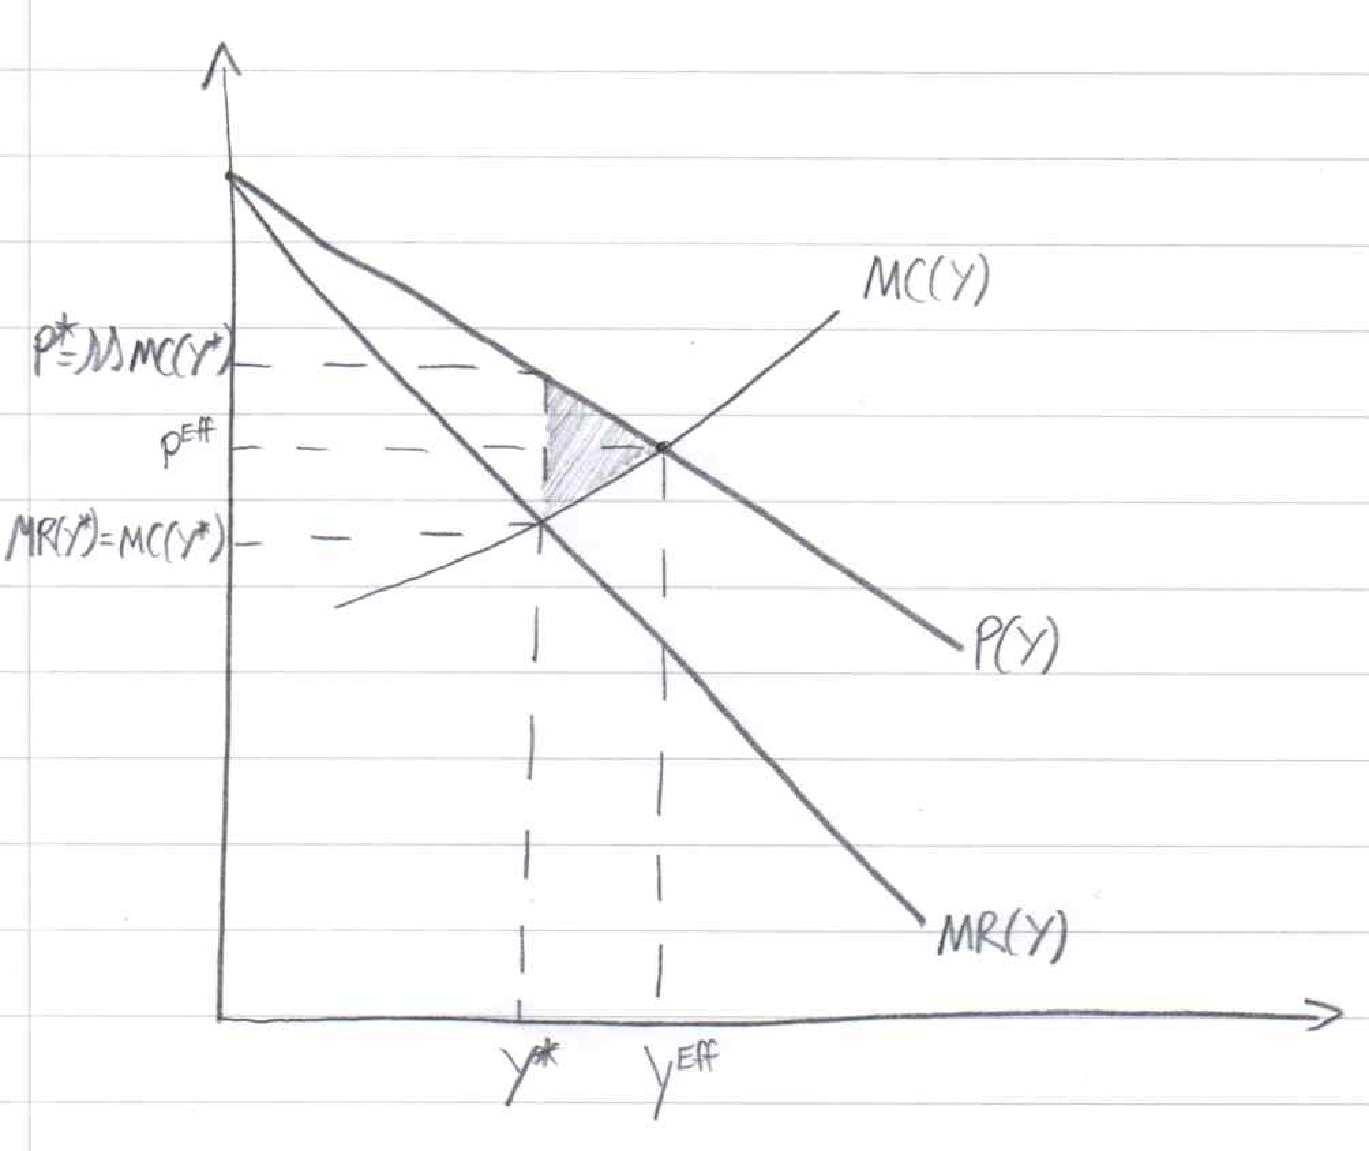
\includegraphics[width=0.6\textwidth]{monop_comp_graph.pdf}}
\caption{\label{fig:monop_comp} Price setting by a firm facing a downward sloping demand curve}
\end{figure}

\end{document}

